\documentclass{article}
\usepackage[a4paper,margin=1.5cm]{geometry}
\usepackage{amsmath,amsfonts}
\usepackage{graphicx}
\usepackage{enumitem}
\usepackage{multicol}
\usepackage{titlesec}
\usepackage{lmodern}
\usepackage{fancyhdr}
\usepackage{hyperref}
\usepackage{multirow}
\usepackage{float}
\usepackage{xparse}
\usepackage{diagbox}
\usepackage{adjustbox}

\titleformat{\section}{\large\bfseries}{\thesection}{1em}{}
\pagestyle{fancy}
\fancyhf{}
\rhead{GATE 2018 – CY}
\lhead{CHEMISTRY}
\rfoot{\thepage}

\title{\textbf{GATE 2018\\Chemistry}}
\date{}

\begin{document}

\maketitle
\noindent \textbf{General Aptitude (GA)}

\section*{Q.1 – Q.5 Carry ONE mark Each}
\begin{enumerate}
\item ``When she fell down the \underline{\hspace{1.5cm}}, she received many \underline{\hspace{1.5cm}} but little help.’’

The words that best fill the blanks in the above sentence are  
\begin{multicols}{2}
\begin{enumerate}
\item stairs, stares
\item stairs, stairs
\item stares, stairs
\item stares, stares
\end{enumerate}
\end{multicols}

\item ``In spite of being warned repeatedly, he failed to correct his \underline{\hspace{2cm}} behaviour.’’

The word that best fills the blank in the above sentence is  
\begin{multicols}{4}
\begin{enumerate}
\item rational
\item reasonable
\item errant
\item good
\end{enumerate}
\end{multicols}

\item For $0 \leq x \leq 2\pi$, $\sin x$ and $\cos x$ are both decreasing functions in the interval \underline{\hspace{2cm}}.  

\begin{multicols}{4}
\begin{enumerate}
\item $(0,\tfrac{\pi}{2})$
\item $(\tfrac{\pi}{2}, \pi)$
\item $(\pi,\tfrac{3\pi}{2})$
\item $(\tfrac{3\pi}{2},2\pi)$
\end{enumerate}
\end{multicols}

\item The area of an equilateral triangle is $\sqrt{3}$. What is the perimeter of the triangle?  

\begin{multicols}{4}
\begin{enumerate}
\item 2
\item 4
\item 6
\item 8
\end{enumerate}
\end{multicols}

\item Arrange the following three-dimensional objects in the descending order of their volumes:  

(i) A cuboid with dimensions $10 \times 8 \times 6$ cm \\ 
(ii) A cube of side 8 cm \\
(iii) A cylinder with base radius 7 cm and height 7 cm \\ 
(iv) A sphere of radius 7 cm  

\begin{multicols}{2}
\begin{enumerate}
\item (i), (ii), (iii), (iv)
\item (ii), (i), (iv), (iii)
\item (iii), (ii), (i), (iv)
\item (iv), (iii), (ii), (i)
\end{enumerate}
\end{multicols}

\section*{Q. 6 – Q. 10 carry two marks each.}
\item An automobile travels from city A to city B and returns to city A by the same route. The speed of the vehicle during the onward and return journeys were constant at 60 km/h and 90 km/h, respectively. What is the average speed in km/h for the entire journey?  

\begin{multicols}{4}
\begin{enumerate}
\item 72
\item 73
\item 74
\item 75
\end{enumerate}
\end{multicols}


\item A set of 4 parallel lines intersect with another set of 5 parallel lines. How many parallelograms are formed?  

\begin{multicols}{4}
\begin{enumerate}
\item 20
\item 48
\item 60
\item 72
\end{enumerate}
\end{multicols}

\item To pass a test, a candidate needs to answer at least 2 out of 3 questions correctly.  
A total of 6,30,000 candidates appeared for the test. \\ 

- Question A was correctly answered by 3,30,000 candidates.  \\
- Question B was answered correctly by 2,50,000 candidates.  \\
- Question C was answered correctly by 2,60,000 candidates.  \\
- Both A and B were answered correctly by 1,00,000 candidates. \\
- Both B and C were answered correctly by 90,000 candidates.  \\
- Both A and C were answered correctly by 80,000 candidates.  \\

If the number of students answering all questions correctly is the same as the number answering none, how many candidates failed to clear the test?  

\begin{multicols}{4}
\begin{enumerate}
\item 30,000
\item 2,70,000
\item 3,90,000
\item 4,20,000
\end{enumerate}
\end{multicols}

\item If $x^2 + x - 1 = 0$, what is the value of $x^4 + \dfrac{1}{x^4}$?  

\begin{multicols}{4}
\begin{enumerate}
\item 1
\item 5
\item 7
\item 9
\end{enumerate}
\end{multicols}

\item In a detailed study of annual crow births in India, it was found that there was relatively no growth during the period 2002 to 2004 and a sudden spike from 2004 to 2005.  
In another unrelated study, it was found that the revenue from cracker sales in India which remained fairly flat from 2002 to 2004, saw a sudden spike in 2005 before declining again in 2006. The solid line in the graph below refers to annual sale of crackers and the dashed line refers to the annual crow births in India. Choose the most appropriate inference from the above data.  

\begin{figure}[h]
    \centering
    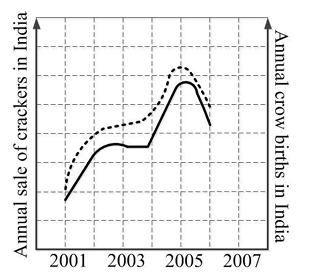
\includegraphics[width=0.5\columnwidth]{figures/asg2 fig1.png}
    \label{fig:placeholder}
\end{figure}

\begin{multicols}{2}
\begin{enumerate}
\item There is a strong correlation between crow birth and cracker sales.  
\item Cracker usage increases crow birth rate.  
\item If cracker sale declines, crow birth will decline.  
\item Increased birth rate of crows will cause an increase in the sale of crackers.  
\end{enumerate}
\end{multicols}
\end{enumerate}

\maketitle
\noindent \textbf{Chemistry (CY)}

\section*{Q. 1 – Q. 25 carry one mark each. }
\begin{enumerate}

\item The major product formed in the following reaction is  

\begin{figure}[H]
\centering
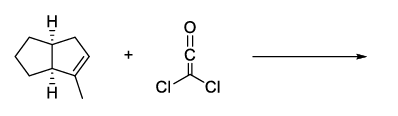
\includegraphics[width=0.5\columnwidth]{figures/cy_q1.png}
\end{figure}

\begin{multicols}{2}
    \begin{enumerate}
        \item \begin{figure}[H]
            \centering
            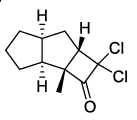
\includegraphics[width=0.5\columnwidth]{figures/cy_q1a.png}
            \label{fig:placeholder}
        \end{figure}

        \item \begin{figure}[H]
            \centering
            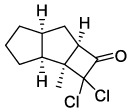
\includegraphics[width=0.5\columnwidth]{figures/cy_q1b.png}
            \label{fig:placeholder}
        \end{figure}

        \item \begin{figure}[H]
            \centering
            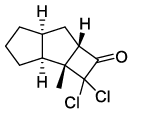
\includegraphics[width=0.5\columnwidth]{figures/cy_q1c.png}
            \label{fig:placeholder}
        \end{figure}

        \item \begin{figure}[H]
            \centering
            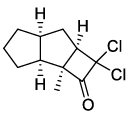
\includegraphics[width=0.5\columnwidth]{figures/cy_q1d.png}
            \label{fig:placeholder}
        \end{figure}
    \end{enumerate}
\end{multicols}

\item The major product formed in the following reaction is
\begin{figure}[H]
    \centering
    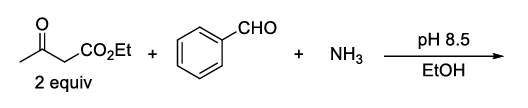
\includegraphics[width=0.6\columnwidth]{figures/cy_q2.png}
    \label{fig:placeholder}
\end{figure}

\begin{multicols}{2}
    \begin{enumerate}
        \item \begin{figure}[H]
            \centering
            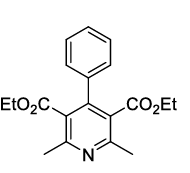
\includegraphics[width=0.4\columnwidth]{figures/cy_q2a.png}
            \label{fig:placeholder}
        \end{figure}

        \item \begin{figure}[H]
            \centering
            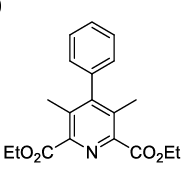
\includegraphics[width=0.4\columnwidth]{figures/cy_q2b.png}
            \label{fig:placeholder}
        \end{figure}

        \item \begin{figure}[H]
            \centering
            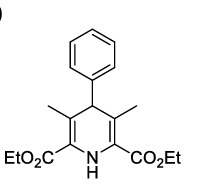
\includegraphics[width=0.4\columnwidth]{figures/cy_q2c.png}
            \label{fig:placeholder}
        \end{figure}

        \item \begin{figure}[H]
            \centering
            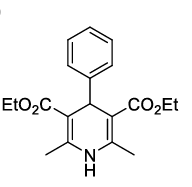
\includegraphics[width=0.4\columnwidth]{figures/cy_q2d.png}
            \label{fig:placeholder}
        \end{figure}
    \end{enumerate}
\end{multicols}

\item The major product of the following intramolecular cycloaddition reaction is
\begin{figure}[H]
    \centering
    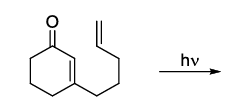
\includegraphics[width=0.3\columnwidth]{figures/cy_q3.png}
    \label{fig:placeholder}
\end{figure}

\begin{multicols}{2}
\begin{enumerate}
    \item \begin{figure}[H]
        \centering
        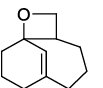
\includegraphics[width=0.3\columnwidth]{figures/cy_q3a.png}
        \label{fig:placeholder}
    \end{figure}

    \item \begin{figure}[H]
        \centering
        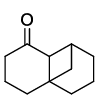
\includegraphics[width=0.3\columnwidth]{figures/cy_q3b.png}
        \label{fig:placeholder}
    \end{figure}

    \item \begin{figure}[H]
        \centering
        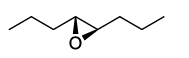
\includegraphics[width=0.3\columnwidth]{figures/cy_q4c.png}
        \label{fig:placeholder}
    \end{figure}

    \item \begin{figure}[H]
        \centering
        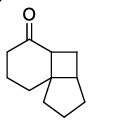
\includegraphics[width=0.3\columnwidth]{figures/cy_q3d.png}
        \label{fig:placeholder}
    \end{figure}
\end{enumerate}
\end{multicols}

\item The major product of the following reaction is
\begin{figure}[H]
    \centering
    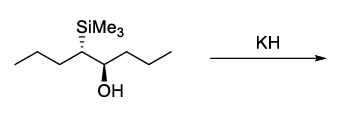
\includegraphics[width=0.4\columnwidth]{figures/cy_q4.png}
    \label{fig:placeholder}
\end{figure}

\begin{multicols}{2}
    \begin{enumerate}
        \item \begin{figure}[H]
            \centering
            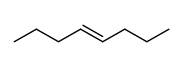
\includegraphics[width=0.4\columnwidth]{figures/cy_q4a.png}
            \label{fig:placeholder}
        \end{figure}

        \item \begin{figure}[H]
            \centering
            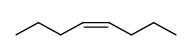
\includegraphics[width=0.4\columnwidth]{figures/cy_q4b.png}
            \label{fig:placeholder}
        \end{figure}

        \item \begin{figure}[H]
            \centering
            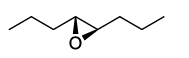
\includegraphics[width=0.4\columnwidth]{figures/cy_q4c.png}
            \label{fig:placeholder}
        \end{figure}

        \item \begin{figure}[H]
            \centering
            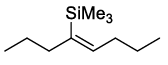
\includegraphics[width=0.4\columnwidth]{figures/cy_q4d.png}
            \label{fig:placeholder}
        \end{figure}
    \end{enumerate}
\end{multicols}

\item The major product formed in the following reaction sequence is
\begin{figure}[H]
    \centering
    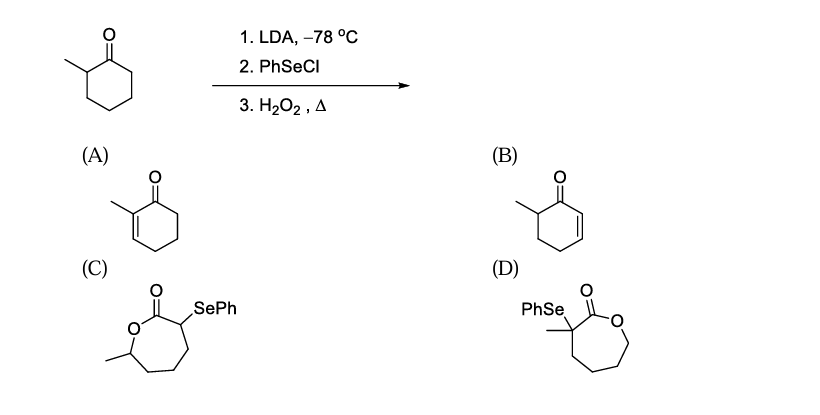
\includegraphics[width=1\columnwidth]{figures/cy_q5.png}
    \label{fig:placeholder}
\end{figure}

\item The major product formed in the following reaction sequence is
\begin{figure}[H]
    \centering
    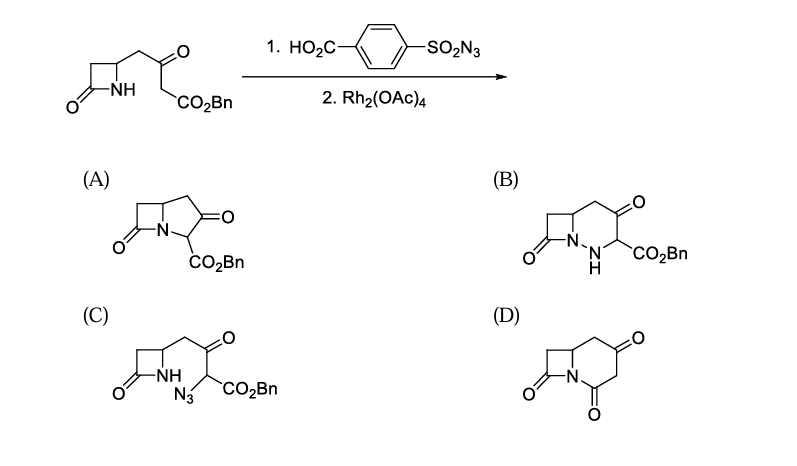
\includegraphics[width=1\columnwidth]{figures/cy_q6.png}
    \label{fig:placeholder}
\end{figure}

\item The spherical harmonic function $Y_l^m(\theta,\phi)$, with appropriate values of $l$ and $m$, 
is an eigenfunction of the operator $\hat{L}_x^2 + \hat{L}_y^2$. 
The corresponding eigenvalue is
\begin{multicols}{4}
\begin{enumerate}
    \item $(l(l+1) - m^2)$
    \item $(l(l+1) + m^2)$
    \item $l(l+1)$
    \item $m^2$
\end{enumerate}
\end{multicols}

% Q8
\item Consider the operators
\[
\hat{a}_+ = \tfrac{1}{\sqrt{2}}\left(\hat{x} + i\hat{p}_x\right), 
\quad 
\hat{a}_- = \tfrac{1}{\sqrt{2}}\left(\hat{x} - i\hat{p}_x\right),
\]
where $\hat{x}$ and $\hat{p}_x$ are the position and linear momentum operators, respectively.  
The commutator $[\hat{a}_+,\hat{a}_-]$ is equal to
\begin{multicols}{2}
\begin{enumerate}
    \item $i$
    \item $-i$
    \item $1$
    \item $-1$
\end{enumerate}
\end{multicols}

% Q9
\item The temperature derivative of electrochemical cell potential $E$ at constant pressure,
$\left(\frac{\partial E}{\partial T}\right)_P$,
 is given by
\begin{multicols}{2}
\begin{enumerate}
    \item $-\dfrac{\Delta S}{nF}$
    \item $\dfrac{\Delta S}{nF}$
    \item $\dfrac{\Delta S}{nFT}$
    \item $-\dfrac{\Delta S}{nFT}$
\end{enumerate}
\end{multicols}

\item For an ionic micelle-forming surfactant near its critical micelle concentration (CMC), the dependence of molar conductivity and surface tension on surfactant concentration is best represented by

\begin{multicols}{2}
    \begin{enumerate}
        \item \begin{figure}[H]
            \centering
            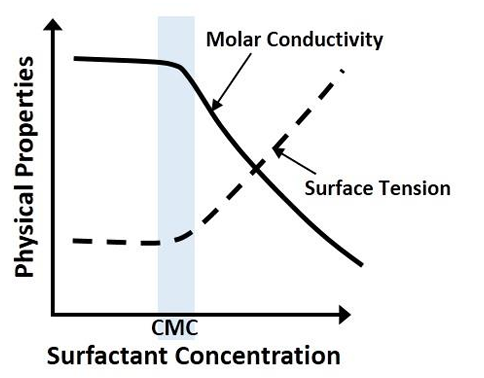
\includegraphics[width=0.4\columnwidth]{figures/cy_q10a.png}
            \label{fig:placeholder}
        \end{figure}

        \item \begin{figure}[H]
            \centering
            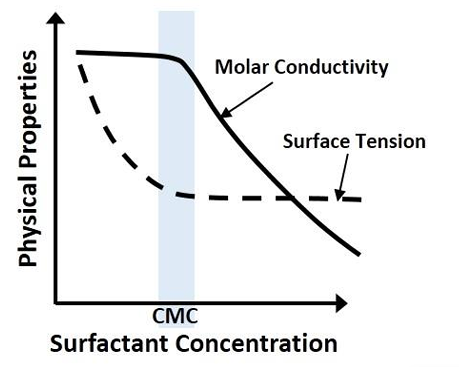
\includegraphics[width=0.4\columnwidth]{figures/cy_10b.png}
            \label{fig:placeholder}
        \end{figure}

        \item \begin{figure}[H]
            \centering
            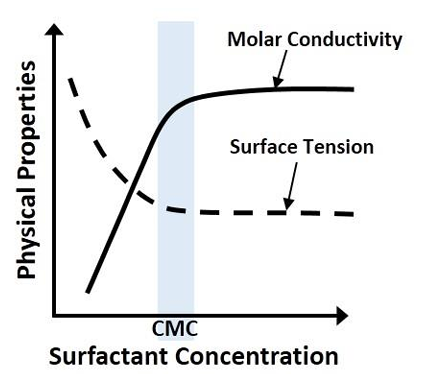
\includegraphics[width=0.4\columnwidth]{figures/cy_10c.png}
            \label{fig:placeholder}
        \end{figure}

        \item \begin{figure}[H]
            \centering
            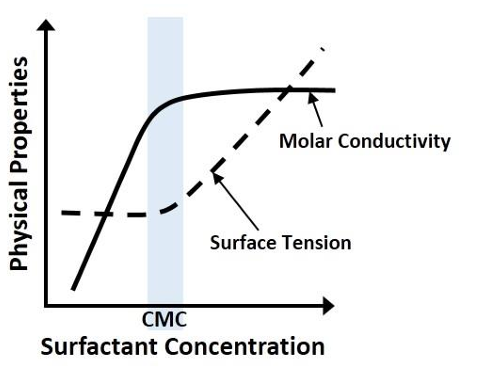
\includegraphics[width=0.4\columnwidth]{figures/cy_10d.png}
            \label{fig:placeholder}
        \end{figure}
    \end{enumerate}
\end{multicols}


\item According to Eyring transition state theory for a bimolecular reaction, the activated 
complex has
\begin{enumerate}
    \item no vibrational degrees of freedom
    \item vibrational degrees of freedom but they never participate in product formation
    \item one high frequency vibration that leads to product formation
    \item one low frequency vibration that leads to product formation
\end{enumerate}

\item Based on Wade’s rule, the structure-type of $[\text{B}_5\text{H}_8]^-$ is
\begin{multicols}{2}
\begin{enumerate}
    \item closo
    \item nido
    \item arachno
    \item hypho
\end{enumerate}
\end{multicols}

\item The coordination geometries around the copper ion of plastocyanin (a blue-copper protein) 
in oxidized and reduced form, respectively, are
\begin{multicols}{2}
\begin{enumerate}
    \item tetrahedral and square-planar
    \item square-planar and tetrahedral
    \item distorted tetrahedral for both
    \item ideal tetrahedral for both
\end{enumerate}
\end{multicols}

\item The water exchange rates for the complex ions follow the order
\begin{multicols}{2}
\begin{enumerate}
    \item $[\text{V(H}_2\text{O)}_6]^{2+} > [\text{Co(H}_2\text{O)}_6]^{2+} > [\text{Cr(H}_2\text{O)}_6]^{3+}$
    \item $[\text{Cr(H}_2\text{O)}_6]^{3+} > [\text{Co(H}_2\text{O)}_6]^{2+} > [\text{V(H}_2\text{O)}_6]^{2+}$
    \item $[\text{Co(H}_2\text{O)}_6]^{2+} > [\text{Cr(H}_2\text{O)}_6]^{3+} > [\text{V(H}_2\text{O)}_6]^{2+}$
    \item $[\text{Co(H}_2\text{O)}_6]^{2+} > [\text{V(H}_2\text{O)}_6]^{2+} > [\text{Cr(H}_2\text{O)}_6]^{3+}$
\end{enumerate}
\end{multicols}

\item The lowest energy d $\rightarrow$ d transition of the complexes follow the order
\begin{multicols}{2}
\begin{enumerate}
    \item $[\text{Cr(H}_2\text{O)}_6]^{3+} < [\text{Cr(NH}_3)_6]^{3+} < [\text{Cr(CN)}_6]^{3-}$
    \item $[\text{Cr(CN)}_6]^{3-} < [\text{Cr(NH}_3)_6]^{3+} < [\text{Cr(H}_2\text{O)}_6]^{3+}$
    \item $[\text{Cr(CN)}_6]^{3-} < [\text{Cr(H}_2\text{O)}_6]^{3+} < [\text{Cr(NH}_3)_6]^{3+}$
    \item $[\text{Cr(NH}_3)_6]^{3+} < [\text{Cr(CN)}_6]^{3-} < [\text{Cr(H}_2\text{O)}_6]^{3+}$
\end{enumerate}
\end{multicols}

\item The symmetry label of valence p orbitals of a metal ion in an octahedral ligand field is
\begin{multicols}{4}
\begin{enumerate}
    \item $t_{1g}$
    \item $t_{1u}$
    \item $e_g + a_{1g}$
    \item $t_{2g}$
\end{enumerate}
\end{multicols}

\item The bond angle (Ti–C–C) in the crystal structure of \\

\begin{figure}[H]
    \centering
    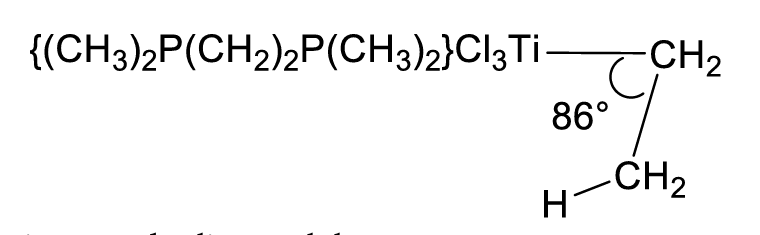
\includegraphics[width=0.5\columnwidth]{figures/cy_q17.png}
    \label{fig:placeholder}
\end{figure}
is severely distorted due to
\begin{multicols}{2}
\begin{enumerate}
    \item hydrogen-bonding interaction
    \item agostic interaction
    \item steric bulk of the phosphine ligand
    \item higher formal charge on metal
\end{enumerate}
\end{multicols}

\item The molar heat capacity of a substance is represented in the temperature range 298 K to 
400 K by the empirical relation $C_{p,m} = bT + 14$ J K$^{-1}$ mol$^{-1}$, where $b$ is a constant.  
The molar enthalpy change when the substance is heated from 300 K to 350 K is 2 kJ mol$^{-1}$.  
The value of $b$ is \underline{\hspace{2cm}} J K$^{-2}$ mol$^{-1}$. (Up to two decimal places)

\item For low partial pressure of ozone (O$_3$), the adsorption of ozone on graphite surface is fully 
dissociative in nature, and follows Langmuir isotherm. Under these conditions, if the 
dependence of the surface coverage of graphite ($\theta$) on partial pressure of ozone ($P_{O_3}$) is 
given by $\theta \propto (P_{O_3})^x$, the value of $x$ is \underline{\hspace{2cm}}. (Up to two decimal places)

\item For the radioactive isotope $^{131}$I, the time required for 50\% disintegration is 8 days.  
The time required for the 99.9\% disintegration of 5.5 g of $^{131}$I is \underline{\hspace{2cm}} days.  
(Up to one decimal place)

\item Two moles of an ideal gas X and two moles of an ideal gas Y, initially at the same 
temperature and pressure, are mixed under isothermal-isobaric condition. The entropy 
change on mixing is \underline{\hspace{2cm}} J K$^{-1}$. (Up to one decimal place. Use $R = 8.31$ J K$^{-1}$ mol$^{-1}$)

\item The energy of a hydrogen molecule in its ground state equilibrium configuration is –31.7 eV.  
Its dissociation energy is \underline{\hspace{2cm}} eV. (Up to one decimal place)

\item The total number of valence electrons in W($\eta^3$-Cp)($\eta^5$-Cp)(CO)$_2$ is \underline{\hspace{2cm}}.  
(Atomic number of W = 74)

\item In the $^1$H NMR spectrum of an organic compound recorded on a 300 MHz instrument, a 
proton resonates as a quartet at $\delta$ 4.20 ppm. The individual signals of the quartet appear  
at $\delta$ 4.17, 4.19, 4.21 and 4.23 ppm. The coupling constant $J$ in Hz is \underline{\hspace{2cm}}.

\item In the electron ionization (EI) mass spectra, methyl hexanoate, methyl heptanoate and methyl 
octanoate give the same base peak. The m/z value of the base peak is \underline{\hspace{2cm}}.

\section*{Q. 26 – Q. 55 carry two marks each.}

\item In the following reaction, 
\begin{figure}[H]
    \centering
    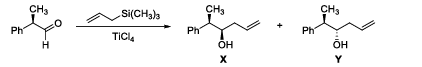
\includegraphics[width=1\columnwidth]{figures/cy_q26.png}
    \label{fig:placeholder}
\end{figure}
\begin{enumerate}
    \item  X is the major product and Y is the minor product
    \item  X is the only product
    \item  Y is the only product 
    \item  X is the minor product and Y is the major product
\end{enumerate}

\item   The enantiomeric pair, among the following, is
\begin{figure}[H]
    \centering
    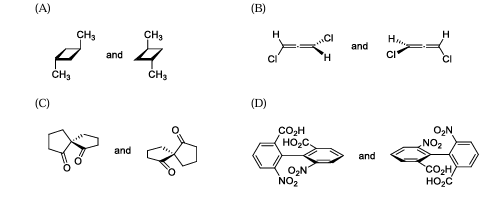
\includegraphics[width=0.9\columnwidth]{figures/cy_q27.png}
    \label{fig:placeholder}
\end{figure}

\item The major product formed in the following reaction sequence is
\begin{figure}[H]
    \centering
    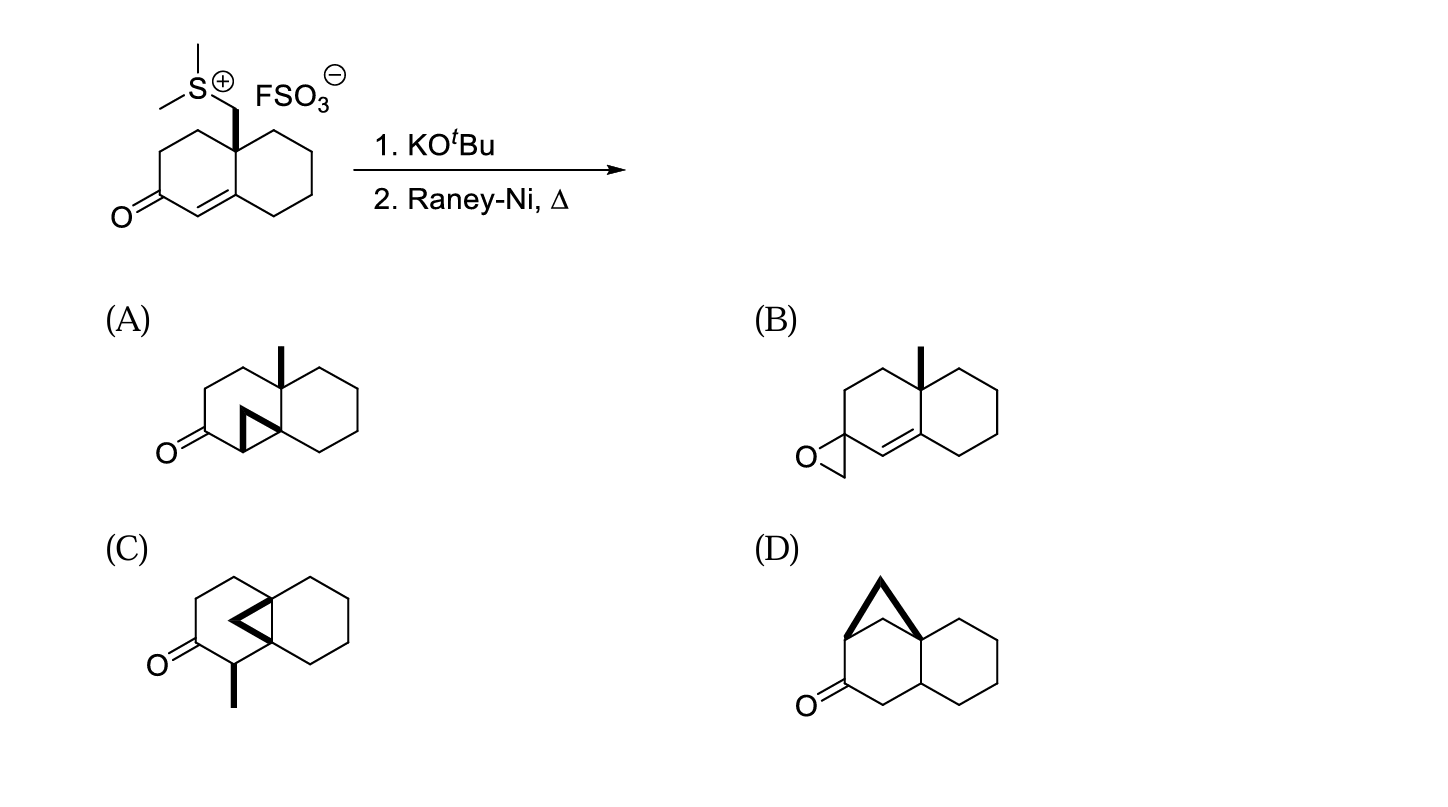
\includegraphics[width=1\columnwidth]{figures/cy_q28.png}
    \label{fig:placeholder}
\end{figure}

\item The major product in the following reaction sequence is
\begin{figure}[H]
    \centering
    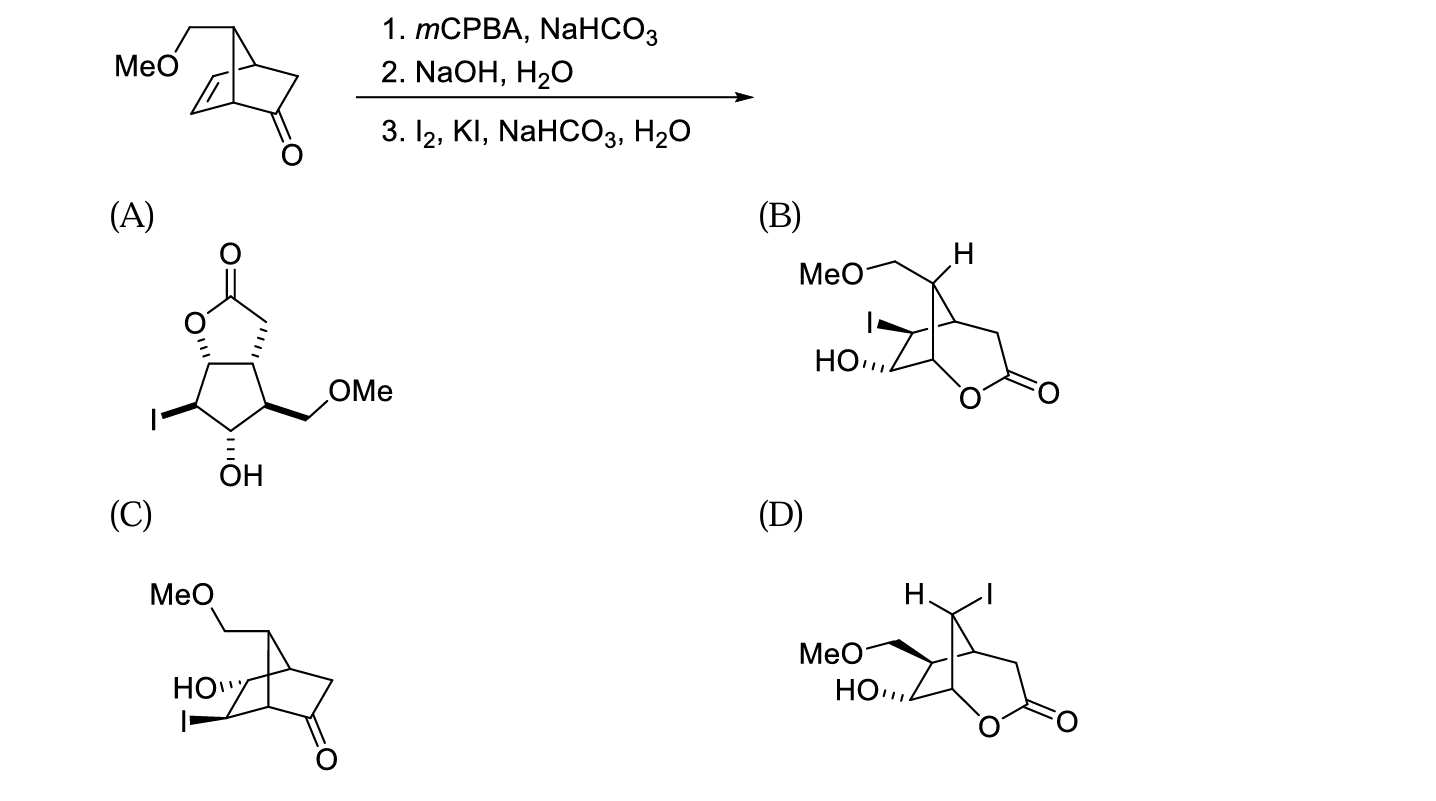
\includegraphics[width=1\columnwidth]{figures/cy_q29.png}
    \label{fig:placeholder}
\end{figure}

\item  The major product formed in the following reaction sequence is 
\begin{figure}[H]
    \centering
    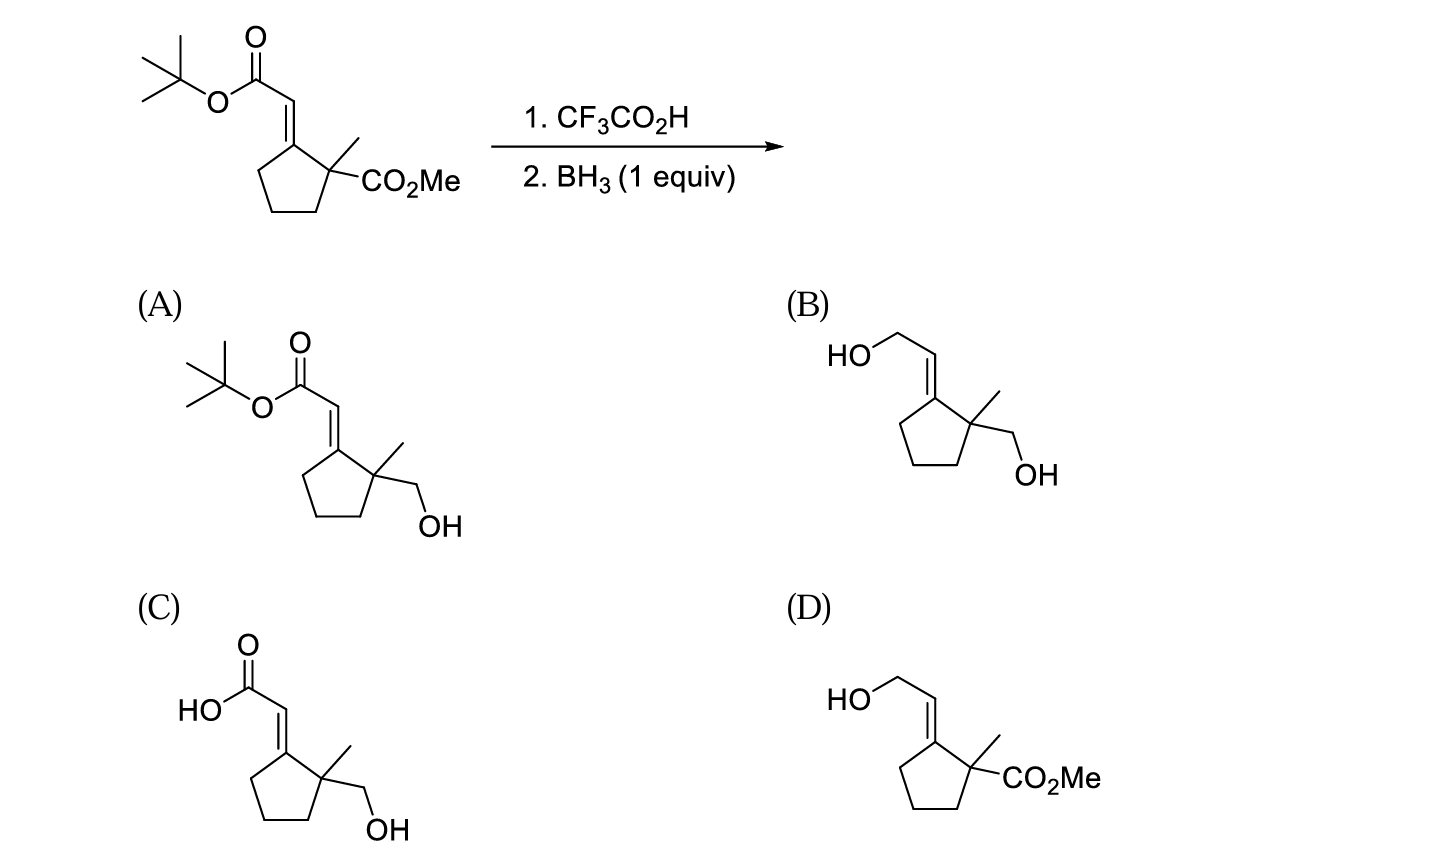
\includegraphics[width=1\columnwidth]{figures/cy_q30.png}
    \label{fig:placeholder}
\end{figure}

\item The major product of the following reaction sequence is
\begin{figure}[H]
    \centering
    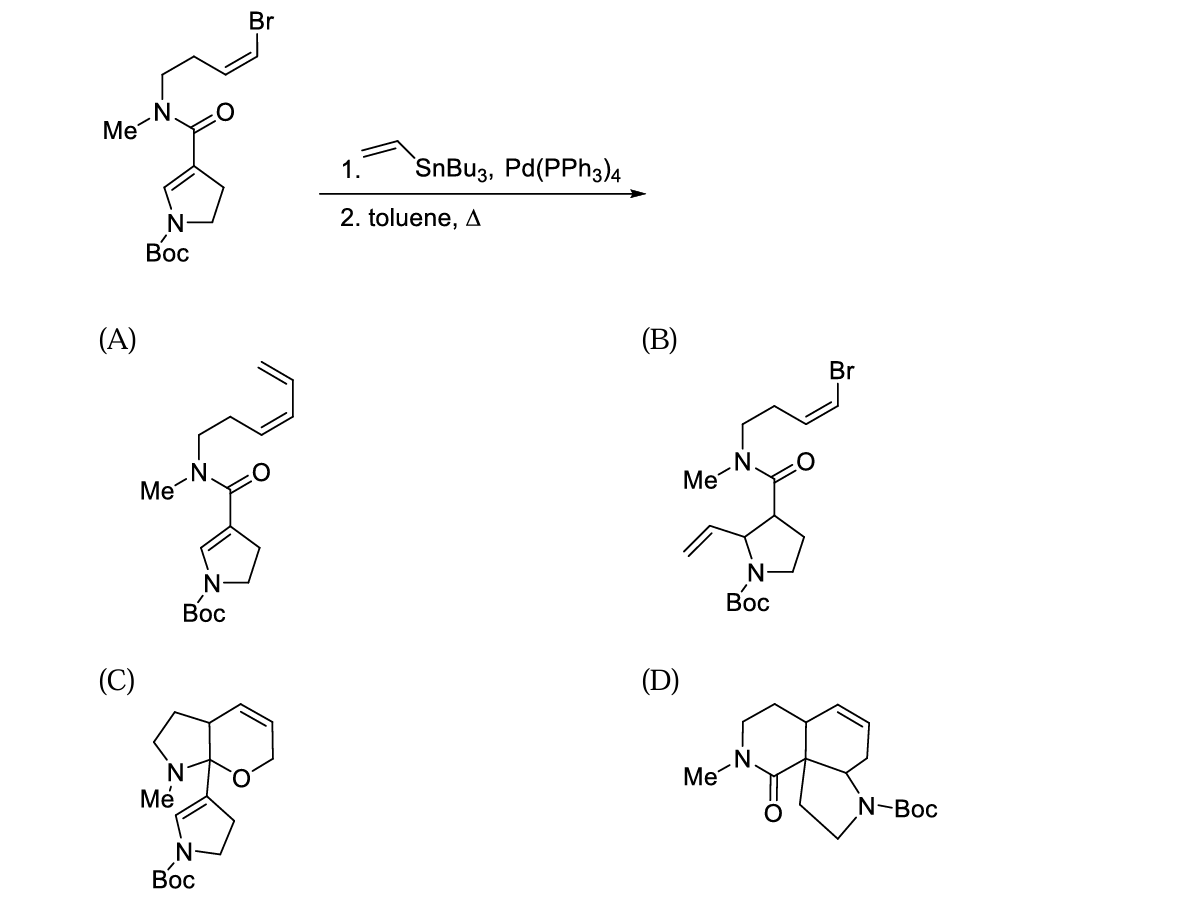
\includegraphics[width=1\columnwidth]{figures/cy_q31.png}
    \label{fig:placeholder}
\end{figure}

\item  The major product formed in the following retro-aldol reaction is
\begin{figure}[H]
    \centering
    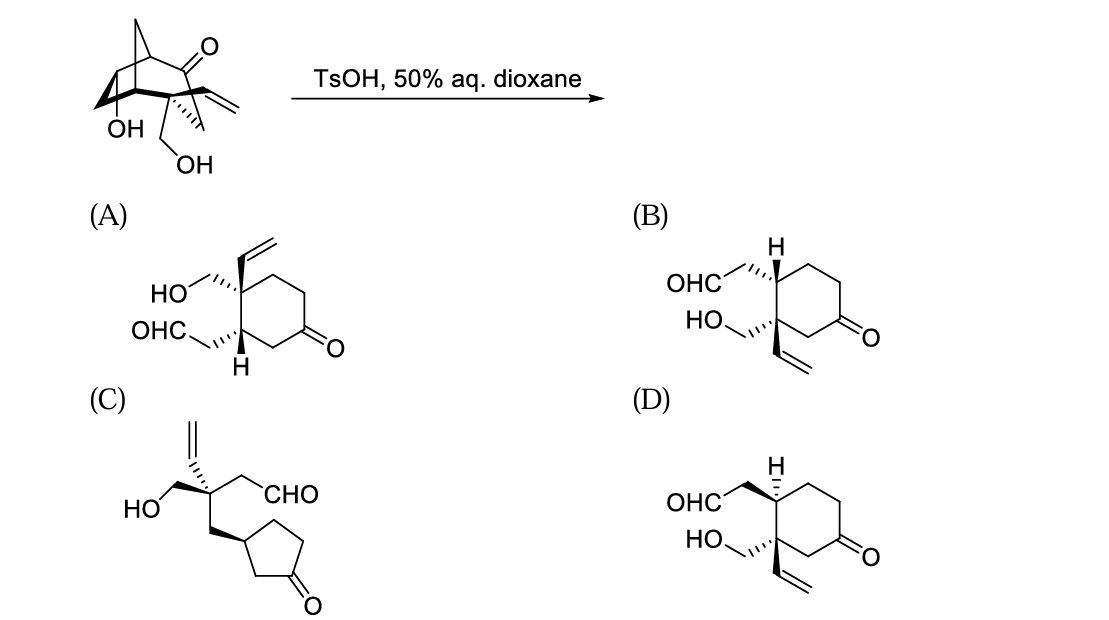
\includegraphics[width=1\columnwidth]{figures/cy_q32.png}
    \label{fig:placeholder}
\end{figure}

\item The major product formed in the following retro-aldol reaction is

\begin{figure}[H]
    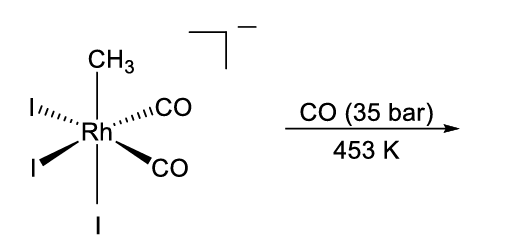
\includegraphics[width=0.4\columnwidth]{figures/cy_q33.png}
    \label{fig:placeholder}
\end{figure}

\begin{multicols}{4}
    \begin{enumerate}
        \item $\text{I}_2$
        \item $\text{CH}_3\text{I}$
        \item $\text{CH}_3\text{COI}$
        \item $\text{I}_3^-$
    \end{enumerate}
\end{multicols}

\item A one-dimensional anharmonic oscillator is treated by perturbation theory. The harmonic 
oscillator is used as the unperturbed system and the perturbation is $\frac{\gamma}{6}x^3$ 
($\gamma$ is a constant). Using only the first order correction, the total ground state energy 
of the anharmonic oscillator is

\begin{multicols}{2}
\begin{enumerate}
    \item $\dfrac{1}{2}\sqrt{\dfrac{k}{\mu}}$
    \item $\dfrac{1}{2}\sqrt{\dfrac{k}{\mu}} + \dfrac{\gamma}{6}\sqrt{\dfrac{1}{\mu k}}$
    \item $\dfrac{1}{2}\sqrt{\dfrac{k}{\mu}} + \dfrac{\gamma}{3}\sqrt{\dfrac{1}{\mu k}}$
    \item $\dfrac{1}{2}\sqrt{\dfrac{k}{\mu}} + \dfrac{\gamma}{12}\sqrt{\dfrac{1}{\mu k}}$
\end{enumerate}
\end{multicols}

\item The O$_2$ coordinated to metal ion centres in oxy-myoglobin and oxy-hemocyanin exists, 
respectively, as
\begin{multicols}{2}
\begin{enumerate}
    \item superoxide and peroxide
    \item superoxide and superoxide
    \item peroxide and peroxide
    \item superoxide and oxygen
\end{enumerate}
\end{multicols}

\item Spectroscopic ground state term symbols of cobalt ions in [Co(H$_2$O)$_6$]$^{2+}$ and [CoCl$_4$]$^{2-}$, 
respectively, are
\begin{multicols}{2}
\begin{enumerate}
    \item $^2T_{1g}$ and $^4A_2$
    \item $^4T_{1g}$ and $^4A_2$
    \item $^4T_{2g}$ and $^4T_1$
    \item $^2T_1$ and $^4A_1$
\end{enumerate}
\end{multicols}

\item Generally, the coordination number and the nature of the electronic absorption band 
(f $\rightarrow$ f transition) of lanthanide(III) ion in their complexes are, respectively,
\begin{multicols}{2}
\begin{enumerate}
    \item greater than 6 and sharp
    \item 6 and broad
    \item less than 6 and sharp
    \item greater than 6 and broad
\end{enumerate}
\end{multicols}

\item Second-order rate constant for the reaction between [Co(NH$_3$)$_5$X]$^{n+}$ 
($n=3$ for X=NH$_3$ and H$_2$O; $n=2$ for X=Cl$^-$) and [Cr(H$_2$O)$_6$]$^{2+}$ 
at room temperature varies with the X as
\begin{multicols}{2}
\begin{enumerate}
    \item NH$_3$ $>$ H$_2$O $>$ Cl$^-$
    \item Cl$^-$ $>$ H$_2$O $>$ NH$_3$
    \item NH$_3$ $>$ Cl$^-$ $>$ H$_2$O
    \item H$_2$O $>$ NH$_3$ $>$ Cl$^-$
\end{enumerate}
\end{multicols}

\item For the following reaction sequence, X and Y, respectively, are
\begin{figure}[H]
    \centering
    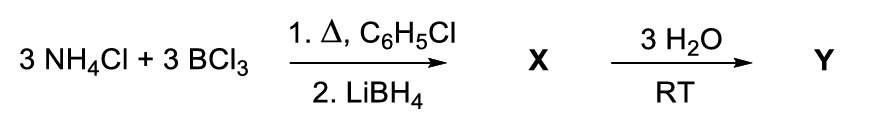
\includegraphics[width=0.5\columnwidth]{figures/cy_q39.png}
    \label{fig:placeholder}
\end{figure}
\begin{multicols}{2}
\begin{enumerate}
    \item \{HB(NH)\}$_3$ and \{H(OH)B(NH$_2$)\}$_3$
    \item \{HB(NH)\}$_3$ and \{HB(NH$_2$OH)\}$_3$
    \item (NH$_4$)\{(H)$_2$(BH$_2$)$_3$\} and \{H(OH)(NH$_2$OH)\}$_3$
    \item (NH$_4$)\{(H)$_2$(BH$_2$)$_3$\} and \{HB(NH$_2$OH)\}$_3$
\end{enumerate}
\end{multicols}

\item For an inverse spinel, AB$_2$O$_4$, the A and B, respectively, can be
\begin{multicols}{2}
\begin{enumerate}
    \item Ni(II) and Ga(III)
    \item Zn(II) and Fe(III)
    \item Fe(II) and Cr(III)
    \item Mn(II) and Mn(III)
\end{enumerate}
\end{multicols}

\item The reaction of PCl$_3$ with PhLi in 1:3 molar ratio yields X as one of the products, which on further treatment with CH$_3$I gives Y. The reaction of Y with n-BuLi gives product Z. The products X, Y and Z, respectively, are
\begin{multicols}{2}
\begin{enumerate}
    \item  \bark[PPh$_4$]Cl, [Ph$_2$P=CH$_2$] and Ph$_2$P(n-Bu)
    \item PPh$_3$, [Ph$_3$PI](CH$_3$) and Ph$_2$P(n-Bu)$_3$
    \item PPh$_3$, [Ph$_3$P(CH$_3$)]I and Ph$_3$P=CH$_2$
    \item \bark[PPh$_4$]Cl, [Ph$_3$P=CH$_2$] and [Ph$_3$P(n-Bu)]Li
\end{enumerate}
\end{multicols}


\item The reaction of equimolar quantities of Fe(CO)$_5$ and OH$^-$ gives a complex species X which 
on further reaction with MnO$_2$ gives species Y. X and Y, respectively, are
\begin{multicols}{2}
\begin{enumerate}
    \item \bark[Fe(CO)$_5$(OH)]$^-$ and Fe$_2$(CO)$_9$
    \item \bark[Fe(CO)$_4$]$^{2-}$ and Mn$_2$(CO)$_{10}$
    \item \bark[HFe(CO)$_4$]$^-$ and Fe$_2$O$_3$
    \item \bark[HFe(CO)$_4$]$^-$ and Fe$_3$(CO)$_{12}$
\end{enumerate}
\end{multicols}

\item The rate constant of a first order reaction, X $\to$ Y, is $1.6\times 10^{-3}$ s$^{-1}$ at 300 K. 
Given that the activation energy of the reaction is 28 kJ mol$^{-1}$ and assuming Arrhenius behavior 
for the temperature dependence, the total time required to obtain 90\% of Y at 350 K 
is \underline{\hspace{2cm}} s. (Up to one decimal place. Use $R = 8.31$ J K$^{-1}$ mol$^{-1}$)

\item The molar conductivity of a 0.01 M weak acid (HX) at 298 K, measured in a conductivity 
cell with cell constant of 0.4 cm$^{-1}$, is 64.4 S cm$^2$ mol$^{-1}$. The limiting molar conductivities at 
infinite dilution of H$^+$ and X$^-$ at 298 K are 350 and 410 S cm$^2$ mol$^{-1}$, respectively. 
Ignoring activity coefficients, the pKa of HX at 298 K is \underline{\hspace{2cm}}. (Up to two decimal places)

\item The Latimer diagram of oxygen is given below. The value of x is \underline{\hspace{2cm}} V. (Up to two decimal places)
\begin{figure}[H]
    \centering
    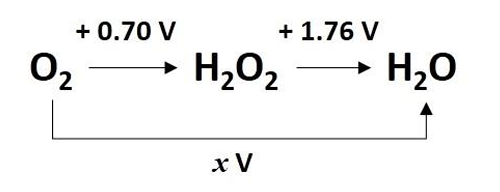
\includegraphics[width=0.5\columnwidth]{figures/cy_q45.png}
    \label{fig:placeholder}
\end{figure}

\item At temperature T, the canonical partition function of a harmonic oscillator with fundamental 
frequency $\nu$ is given by
\[
q_{\text{vib}}(T) = \frac{e^{-h\nu/2k_BT}}{1 - e^{-h\nu/k_BT}}
\]
For $\dfrac{h\nu}{k_BT} = 3$, the probability of finding the harmonic oscillator in its ground 
vibrational state is \underline{\hspace{2cm}}. (Up to two decimal places)

\item The enthalpy of vaporization of a liquid at its boiling point ($T_b = 200$ K) is 15.3 kJ mol$^{-1}$. 
If the molar volumes of the liquid and the vapour at 200 K are 110 and 12000 cm$^3$ mol$^{-1}$ 
respectively, then the slope $\dfrac{dP}{dT}$ of the liquid-vapour boundary is \underline{\hspace{2cm}} kPa K$^{-1}$. 
(Up to two decimal places. Note: 1 Pa = 1 J m$^{-3}$)

\item In a molecule XY, let $\psi_X$ and $\psi_Y$ denote normalized atomic orbitals of atoms X and Y, 
respectively. A normalized molecular orbital of XY is given by 
$\psi = 0.56(\psi_X + \psi_Y)$.  
The value of the overlap integral of $\psi_X$ and $\psi_Y$ is \underline{\hspace{2cm}}. (Up to two decimal places)

\item The absorption maxima of two dyes X and Y are 520 and 460 nm, respectively. The absorbance data of these dyes measured in a 1 cm path length cell are given in the table below:

\begin{center}
\begin{tabular}{|c|c|c|}
\hline
Dye solution & Absorbance at 460 nm & Absorbance at 520 nm \\
\hline
 X (9 mM) & 0.144 & 0.765 \\
Y (12 mM) & 0.912 & 0.168 \\
Mixture of X and Y & 0.700 & 0.680 \\
\hline
\end{tabular}
\end{center}

The concentration of Y in the mixture is \underline{\hspace{2cm}} mM. (Up to two decimal places)

\item The $\pi$ electrons in benzene can be modelled as particles in a ring that follow Pauli’s 
exclusion principle. Given that the radius of benzene is 1.4 \AA, the longest wavelength of light 
that is absorbed during an electronic transition in benzene is \underline{\hspace{2cm}} nm.  
(Up to one decimal place. Use $m_e=9.1\times 10^{-31}$ kg, $h=6.6\times 10^{-34}$ J s, $c=3.0\times 10^8$ m s$^{-1}$)

\item The spacing between the two adjacent lines of the microwave spectrum of H$^{35}$Cl is 
$1.1635\times 10^{11}$ Hz. Given that the bond length of D$^{35}$Cl is 5\% greater than that of H$^{35}$Cl, 
the corresponding spacing for D$^{35}$Cl is \underline{\hspace{2cm}} $\times 10^{10}$ Hz. (Up to two decimal places)

\item For a diatomic vibrating rotor, in vibrational level $\nu=3$ and rotational level J, the sum of 
the rotational and vibrational energies is 1493.6 cm$^{-1}$. Its equilibrium oscillation frequency is 
2998.3 cm$^{-1}$, anharmonicity constant is 0.0124 and rotational constant under rigid rotor 
approximation is 9.716 cm$^{-1}$. The value of J is \underline{\hspace{2cm}}. (Up to nearest integer)

\item Number of carbonyl groups present in the final product of the following reaction sequence is \underline{\hspace{2cm}}.
\begin{figure}[H]
    \centering
    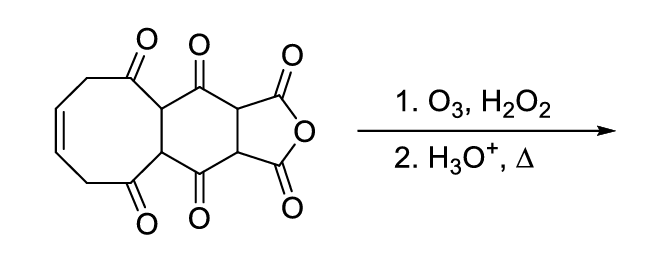
\includegraphics[width=0.5\columnwidth]{figures/cy_q53.png}
    \label{fig:placeholder}
\end{figure}

\item A tetrapeptide, made up of natural amino acids, has alanine as the N-terminal residue 
which is coupled to a chiral amino acid. Upon complete hydrolysis, the tetrapeptide gives 
glycine, alanine, phenylalanine and leucine. The number of possible sequences of the 
tetrapeptide is \underline{\hspace{2cm}}.

\item The strongest band observed in the IR spectrum of the final product of the following 
reaction appears, approximately, at \underline{\hspace{2cm}} $\times 100$ cm$^{-1}$. (Up to one decimal place)
\begin{figure}[H]
    \centering
    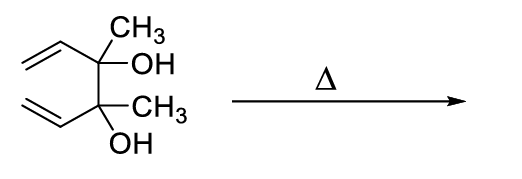
\includegraphics[width=0.5\columnwidth]{figures/cy_q55.png}
    \label{fig:placeholder}
\end{figure}

\end{enumerate}
\end{document}

